\documentclass[twoside,11pt]{article}

\title{IEOR 4500 Application Programming for FE \\
  \large Assignment 1
} % DON'T CHANGE THIS

\author{Anurag Dutt, Shrey Goel, Jatindeep Singh, Vinayak Shinde, Aditya Zalte}    % YOUR NAME GOES HERE
%\studmail{}% YOUR UNI GOES HERE
%\hwNo{1}                   % THE HOMEWORK NUMBER GOES HERE
%\collab{Group 19}   % THE UNI'S OF STUDENTS YOU DISCUSSED WITH

% Uncomment the next line if you want to use \includegraphics.
\usepackage{graphicx}

\begin{document}
\maketitle
This file includes te write-up and explanations for any of the problems in the aforementioned assignment

\section*{Problem 2}
% YOUR SOLUTION GOES HERE
For handling the missing values, we arranged the returns matrix	based on ascending order of time. The oldest values on top and the most	recent values towards the last.	Then we	applied	forward filling of the NA values such	that corresponding cells took the returns of the previous date.	We could also have done	mean imputation	where the cells	containing NA values could have	beenfilled with the mean of the previous and	the next day's returns,	but we didn't do mean imputation because it wouldn't have made sense to	incorporate the	future values into imputation of NA values. Hence we chose to stick with forward filling process.

The formula used for variance for jth security was (diagonal elements of the covariance matrix - 947 securities and 504 days):-
\begin{equation}
  Var(x_j) = \sigma_x^2 = \sum_{i = 1}^{504} (\mu_{ij}-\overline{\mu})^2
\end{equation}

The covariance between jth and kth security was calculated as:-
\begin{equation}
  Cov(x_jx_k) = \sum_{i = 1}^{504} (\mu_{ij}-\overline{\mu_j})(\mu_{ik}-\overline{\mu_k})
\end{equation}

For optimization purposes, we calculated the upper triangle of the covariance matrix and used it fill the lower triangle.

\section*{Problem 3}
% YOUR SOLUTION GOES HERE

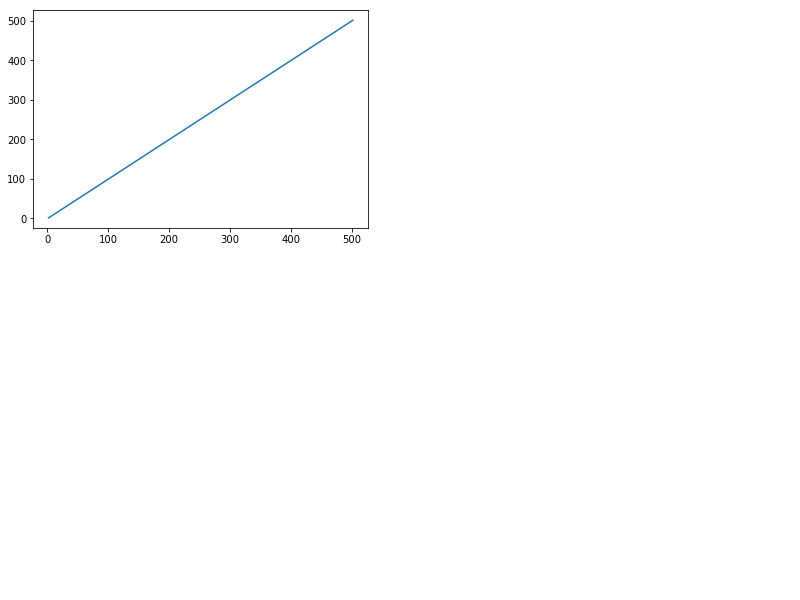
\includegraphics{graph_q3.png}

\section*{Problem 4}
% YOUR SOLUTION GOES HERE
We used	$A^2$ instead of $A$ and it drastically reduced the runtime by almost 5. Thr initial runtime was 5.1 secs which reduced to 0.9 secs.


\end{document} 
